\documentclass[tikz,convert,convert={outext=.pdf,command=\unexpanded{}}]{standalone}

\usepackage{array}
\usepackage{amsmath,mathrsfs,xcolor,circledtext}
\usepackage{graphicx}
\usepackage{tikz}
\usepackage{tikz-3dplot}
\usepackage{ctex}
\usepackage{circledtext}
\usepackage{pgfplots}
\usepackage[american]{circuitikz}
\usetikzlibrary{decorations.pathreplacing,calc,quotes,angles}
\pgfplotsset{compat=1.15}
\usepgfplotslibrary{polar}


\newcommand \lightblue {cyan!20}
\newcommand \lightred {red!20}

\tdplotsetmaincoords{75}{105}
%视角旋转命令:\tdplotsetmaincoords{num}{num}
%含义:{绕x轴顺时针旋转<num>度}{绕y轴顺时针旋转<num>度}
%普通的右手系设定为{60}{120},即绕x轴顺时针旋转60°,绕y轴顺时针旋转120°

\begin{document}
    \centering
    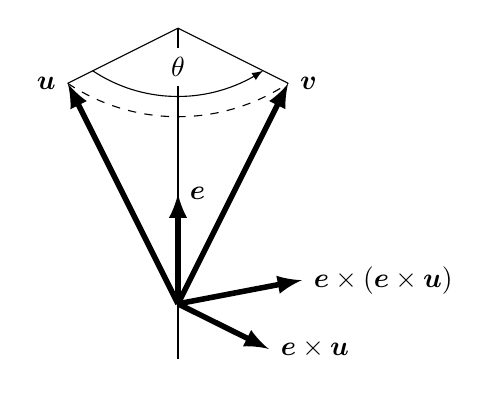
\begin{tikzpicture}[
        scale = 0.7,
        >= latex
    ]
        \draw (0,-2)-- (0,4);
        \draw [->,line width=2pt] (0,-1)--(0,1)node[right]{$\boldsymbol{e}$};
        \draw [->,line width=2pt] (0,-1)--(1.65,-1.82)node[right]{$\boldsymbol{e}\times \boldsymbol{u}$};
        \draw [->,line width=2pt] (0,-1)--(2.25,-0.57)node[right]{$\boldsymbol{e}\times \left( \boldsymbol{e}\times \boldsymbol{u} \right) $};
        \draw [dashed](-2,3) arc (236.3099325:303.6900675:3.605551275);
        \draw [->](-1.55,3.23) arc  (236.3099325:303.6900675:2.79);
        \node [fill = white]at (0,3.3) {$\theta $};
        \draw (0,4)-- (-2,3);
        \draw (0,4)-- (2,3);
        \draw [->,line width=2pt] (0,-1)--(-2,3)node[left]{$\boldsymbol{u}$};
        \draw [->,line width=2pt] (0,-1)--(2,3)node[right]{$\boldsymbol{v}$};
        \end{tikzpicture}
\end{document}